Let $y$ be the position of a particle in one dimension, and let $t$ be time. So
there is just a single input variable: $t$.

An Ordinary Differential Equation is an equation relating the input variable
$t$ to $y$ and its derivatives. So, in general,
\begin{align*}
  f\(t, y, y', y'', \ldots\) = 0.
\end{align*}

A first-order ODE involves first derivatives only.

Consider the subset\footnote{I.e. $f(t, y, y') = 0$ can be rearranged to give
  $y'$ as a function of $t, y$.} of first-order ODEs that specify a velocity
$v(t, y)$ at each point in $(t, y)$ space. Thus this ODE contains all the
information needed to animate the motion of the particle, starting from any
point $(t_0, y_0)$. So the statement of the initial condition problem is
\begin{align*}
  \dydt = v(t, y) ~~~~~~~~~~ y(t_0) = y_0.
\end{align*}

The solution to an ODE is a function $y = \varphi(t)$ that describes a motion
of the particle having the specified velocities at each point it passes
through. I.e., if $y = \varphi(t)$ is a solution, then
\begin{align*}
  \frac{\d \varphi}{\dt} = v\Big(t, \varphi(t)\Big) ~~~~~~~~~~~~~\text{for all $t$}.
\end{align*}

We can think of $v$ as a surface over the $(t, y)$ plane. A solution is a curve
in the plane whose derivative is equal to the height of the surface $v$, at
every point on the curve.

The phase space of this problem is the set of all possible $(y, v)$ values.?

\section{Special cases}
\subsection{Velocity depends on time only}
\begin{align*}
  \dydt = v(t)
\end{align*}
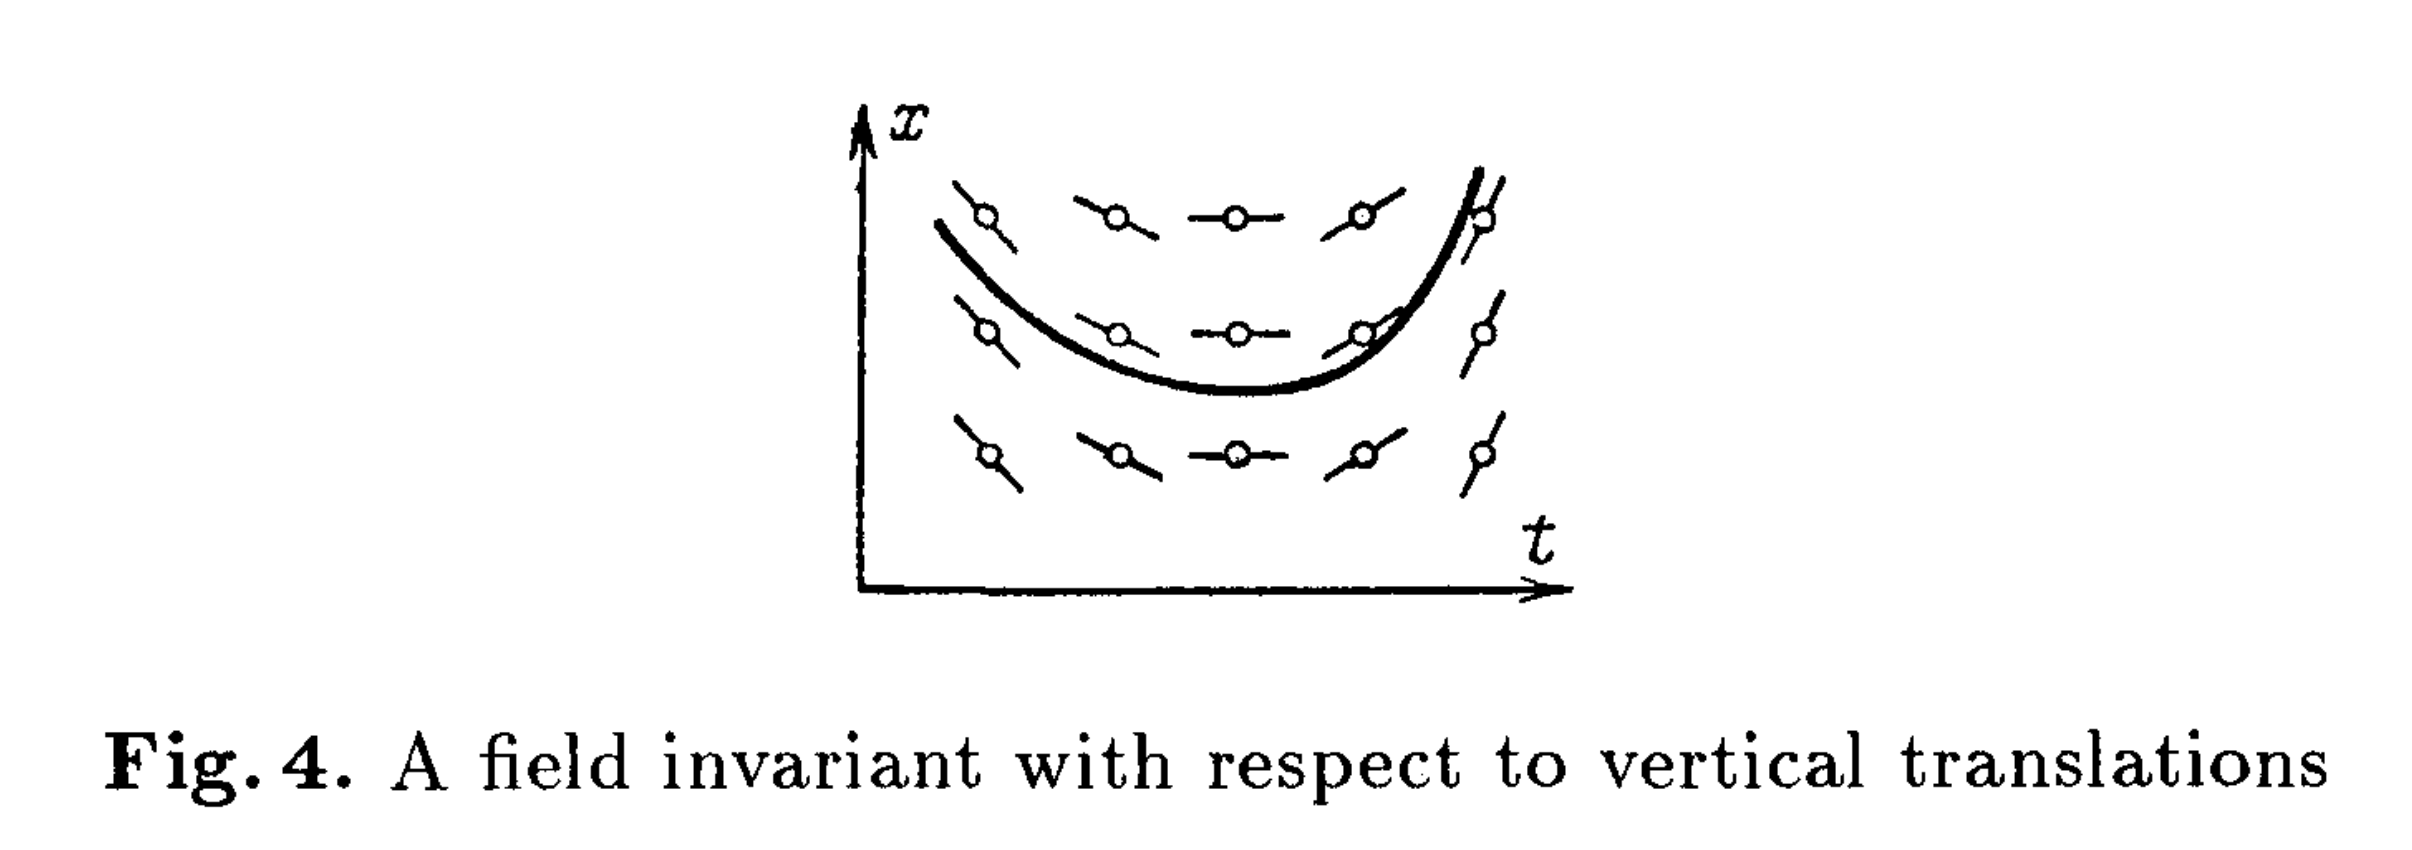
\includegraphics[width=340pt]{img/differential-equations-1-direction-field.png}\\
To find functions that solves this, one possibility is that we can find the
antiderivative explicitly:
\begin{align*}
  \int \dydt \dt := y(t) + C = \int v(t) \dt.
\end{align*}


\subsection{Velocity depends on location only (autonomous)}
\begin{align*}
  \dydt = v(y)
\end{align*}
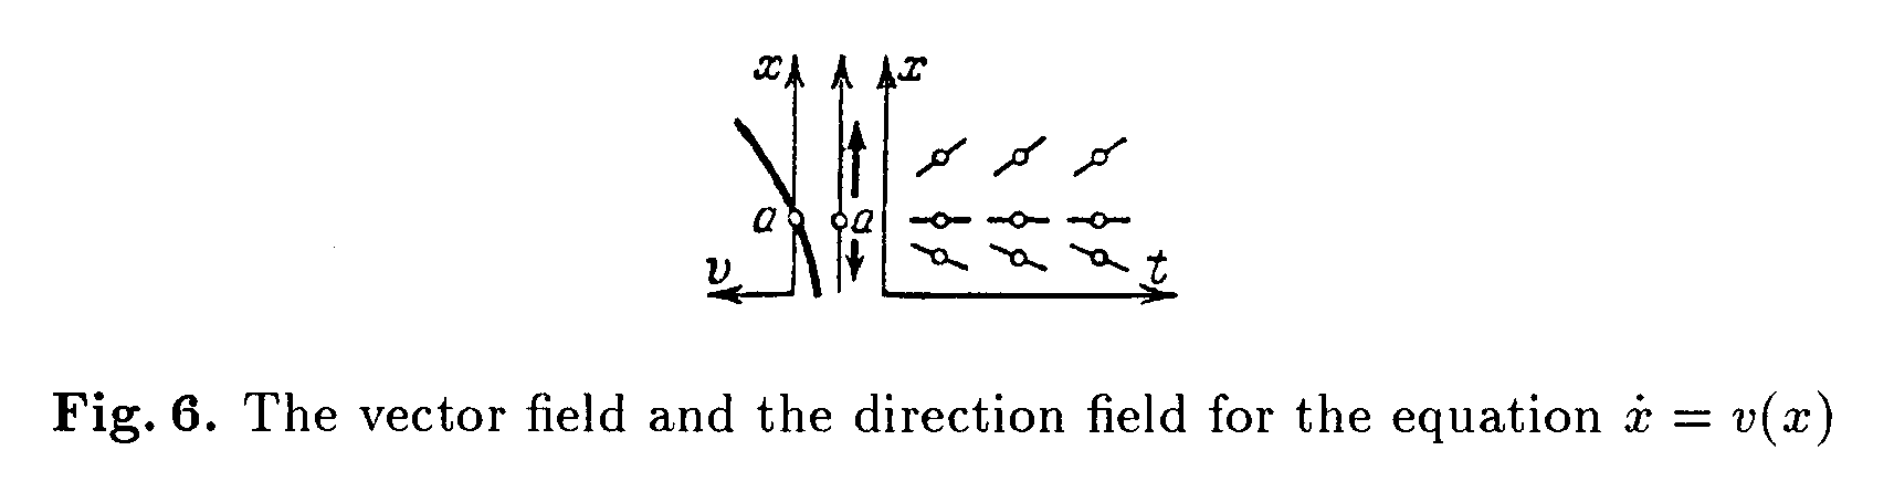
\includegraphics[width=400pt]{img/differential-equations-2-direction-field.png}\\



\section{Examples}
\subsection{C$^{14}$ dating}
\begin{mdframed}
  In a living organism the amount of C$^{14}$, as a proportion of all the
  C$^{12}$ and C$^{14}$, is expected to be a known constant $p_0$. After death,
  C$^{14}$ decays to C$^{12}$. How old is a specimen with proportion $p_1$ of
  C$^{14}$?
\end{mdframed}
Let $\lambda$ be the rate at which one atom of C$^{14}$ decays in atoms/sec. So
in a sample of $N$ atoms, the expected number to decay in one second is
$N\lambda$.

Let $N(t)$ be the number of C$^{14}$ atoms remaining at time $t$. We can
specify the model as a first-order ODE:
\begin{align*}
\frac{\d N}{\dt} = -N\lambda.
\end{align*}
Equivalently, dividing by the constant total number of carbon atoms,
\begin{align*}
\frac{\d p}{\dt} = -p\lambda,
\end{align*}
where $p(t)$ is the proportion of C$^{14}$ at time $t$.

It's easy to find a family of functions $p(t)$ that satisfies this differential equation. Since
\begin{align*}
  \frac{1}{p(t)} \frac{\d p}{\dt} = -\lambda,
\end{align*}
it must be the case that their antiderivatives are the same, up to a constant:
\begin{align*}
  \log(p(t)) &= -\lambda t + C\\
  p(t)  &= Ae^{-\lambda t}.
\end{align*}
Further, the expected proportion in a living organism determines a particular
function as the solution:
\begin{align*}
  p(0) = p_0 = Ae^{-\lambda . 0}
\end{align*}
so $A = p_0$ and the solution is
\begin{align*}
  p(t)  &= p_0e^{-\lambda t}.
\end{align*}
So the estimated age of a sample with proportion $p_1$ is
\begin{align*}
  t = \frac{1}{\lambda}\log\(\frac{p_0}{p_1}\).
\end{align*}



\section{Picard's Existence Theorem}
Consider again the initial value problem
\begin{align*}
  \dydt = v(t, y) ~~~~~~~~~~ y(t_0) = y_0.
\end{align*}


The ODE could also be written as
\begin{align*}
  y(t) = \int v\Big(t, y(t)\Big) \dt + C,
\end{align*}
but this is merely an equivalent restatement, since the definition of
indefinite integral is antiderivative. If we can find an antiderivative, then
fine. If not, note that by FTC, the following definite integral describes a
solution:
\begin{align*}
  y(t) = y(t_0) + \int_{t_0}^t v\Big(\tau, y(\tau)\Big) \d\tau.
\end{align*}
But this specifies $y(t)$ in terms of itself, since the velocity $v$ depends
not only on $t$ but also on the current position\footnote{for example, the rate
  of change of the proportion on carbon-14 depends on the current proportion of
  carbon-14.}.\\

\subsection{Definition: Lipschitz condition}
$v(t, y)$ is Lipschitz in the $y$ direction if there exists an upper bound $L$
on the absolute value of the straight line slope between any two points lying
on a vertical line. I.e. $\exists L > 0$ such that
\begin{align*}
  \Big|v(t, y_1) - v(t, y_0)\Big| \leq L\Big|y_1 - y_0\Big|
\end{align*}
for all pairs of points $(t, y_0)$, $v(t, y_1)$.

\subsection{Theorem: Picard's existence theorem}
\begin{mdframed}
Let $R$ be a rectangle of width $2h$ and height $2k$ and let
$(t_0, y_0)$ be the center of the rectangle. Suppose
\begin{enumerate}
\item Within $R$, $v(t, y)$ is continuous, with $|v(t, y)| \leq M$
\item $Mh \leq k$
\item Within $R$, $v(t, y)$ is Lipschitz in the $y$ direction, with bound $L$
  on the absolute value of the straight line slope between any two points.
\end{enumerate}

Then the initial value problem
\begin{align*}
  \dydt = v(t, y) ~~~~~~~ y(t_0) = y_0
\end{align*}
has a unique solution in $R$.
\end{mdframed}

\subsection{Examples}

In these cases, $|y'|$ and $\partiald{v}{y}$ are bounded in any rectangle.

\subsubsection{A}
$y' = v(x, y) = x^2 + y^2 ~~~~~~~ y(0) = 0$

So it can be approximated by Picard iterates. Is an explicit solution possible here?

\subsubsection{B}
$y' = (1 - 2x)y ~~~~~~~ y(0) = 1$

This can be solved explicitly by separation-of-variables:
\begin{align*}
  \log(y) &= x- x^2 + C\\
  y       &= Ae^{x(1-x)}.
\end{align*}


\subsection{Non-examples}

$|y'|$ is bounded in any rectangle for all these examples. However,
$\partiald{v}{y}$ is not. Picard's theorem guarantees unique solutions only in
rectangles excluding such problematic points.

\subsubsection{A}
$y' = v(x, y) = 3y^{2/3}  ~~~~~~~ y(0) = 0$

$\partiald{v}{y} = 2y^{-1/3} \to \pm \infty$ at $y=0$.


\subsubsection{B}
$y' = v(x, y) = x^2y^{1/5} ~~~~~~~ y(0) = b$

$\partiald{v}{y} = \frac{1}{5}x^2y^{-4/5}$ which is not defined at $y=0$.

\subsubsection{C}
$y' = v(x, y) = y^2       ~~~~~~~ y(0) = 1$

$\partiald{v}{y} = 2y$, so seems like it should be fine. Solve by
separation-of-variables:

\begin{align*}
  \int y^{-2} y' \dx &= x + C\\
  -y^{-1}            &= x + C\\
  y                 &= \frac{1}{C - x}.
\end{align*}
The solution passing through the initial value $y(0) = 1$ is
\begin{align*}
  y                  &= \frac{1}{1 - x},
\end{align*}
which does not exist for all $x$ in the rectangle.


\newpage
\subsection{Proof}

We will show that the following sequence of functions converges to a unique
solution:
\begin{align*}
  y_0(t) &= y_0\\
  y_n(t) &= y_0 + \int_{t_0}^t v\Big(\tau, y_{n-1}(\tau)\Big) \d\tau.\\
\end{align*}

The basic idea is to write the limiting function $y_\infty(t)$ as a telescoping
sum, and then to show that the series thus defined converges.

Define
\begin{align*}
  e_n = y_n - y_{n-1}, ~~~~~~~ n = 1, 2, \ldots.
\end{align*}
Then the limiting function that is our objective is
\begin{align*}
  y_\infty = y_0 + \sum_{n=1}^\infty e_n.
\end{align*}

We need to show
\begin{enumerate}
\item The $y_n(t)$ converge to a function $y(t)$
\item This function is a solution
\item It is unique
\end{enumerate}

\newpage
\subsection{Proof that the $y_n(t)$ converge uniformly to a function $y_\infty(t)$}
We are going to use the Weierstrass M-test to show that the series of functions
converge uniformly. So, we need to show that each $e_n$ is bounded
by some $W_n$, and that the series $\sum_{n=1}^\infty W_n$ converges.

A single term in the series is
\begin{align*}
  e_{n}(t) = \int_{t_0}^t v\Big(\tau, y_{n-1}(\tau)\Big) -
                         v\Big(\tau, y_{n-2}(\tau)\Big) \dt.
\end{align*}

Now, by assumption, $v$ is Lipschitz in the $y$ direction with bound
$L$. (Informally, this means that the absolute value of the straight line slope
between any two points lying on a vertical line is bounded by $L$). Therefore
\begin{align*}
  \Big|v\Big(t, y_{n-1}(t)\Big) -
       v\Big(t, y_{n-2}(t)\Big)\Big| \leq L\Big|y_{n-1}(t) - y_{n-2}(t)\Big|.
\end{align*}
And since $\Big|\int_a^b f(t) \dt\Big| \leq \int_a^b |f(t)| \dt$,
\begin{align*}
  |e_n(t)| \leq L\Big|\int_{t_0}^t \Big|y_{n-1}(\tau) - y_{n-2}(\tau)\Big| \d\tau \Bigg|.
\end{align*}
\footnote{The outer modulus is required to handle the case $t < t_0$.}

For the Weierstrass M-test we need to express the RHS as a constant $W_n$,
depending only on $L, M, n, t_0, y_0$. We will do this by induction.

\newpage
Recall that the definition of the $e_n$ is
\begin{align*}
  e_n(t) := y_n(t) - y_{n-1}(t).
\end{align*}

For the first few terms we have
\begin{align*}
  |e_1(t)| &    = \int_{t_0}^t v(\tau, y_0) \d\tau\\
           & \leq M(t - t_0) \leq Mh\\
  |e_2(t)| & \leq L\int_{t_0}^t \Big|y_1(\tau) - y_0(\tau)\Big| \d\tau\\
           &    = L\int_{t_0}^t |e_1(\tau)| \d\tau\\
           & \leq L\int_{t_0}^t M(\tau - t_0) \d\tau\\
           &    = LM\frac{(\tau - t_0)^2}{2} \Big|_{t_0}^t \\
           &    = LM\frac{(t - t_0)^2}{2} \\
  |e_3(t)| & \leq L\int_{t_0}^t \Big|y_2(\tau) - y_1(\tau)\Big| \d\tau\\
           &    = L\int_{t_0}^t |e_2(\tau)| \d\tau\\
           & \leq L\int_{t_0}^t LM\frac{(t - t_0)^2}{2} \d\tau\\
           &    = L^2M\frac{(t - t_0)^3}{3!}
\end{align*}
So it seems that $|e_n(t)| \leq L^{n-1}M\frac{h^n}{n!}$. To prove this, note that we know
it is true of $e_1$. So suppose it is true of $e_n$. Then the next term is
\begin{align*}
  e_{n+1}(t) &   := y_{n+1}(t) - y_n(t)\\
            & \leq L\int_{t_0}^t \Big|y_n(\tau) - y_{n-1}(\tau)\Big| \d\tau\\
            &=     L\int_{t_0}^t |e_n(\tau)| \d\tau\\
            &=     L\int_{t_0}^t L^{n-1}M\frac{(\tau - t_0)^n}{n!} \d\tau\\
            &=     L^nM\frac{(t - t_0)^{n+1}}{(n+1)!^{~~~}}\\
            & \leq L^nM\frac{h^{n+1}}{(n+1)!},
\end{align*}
so $|e_n(t)| \leq L^{n-1}M\frac{h^n}{n!}$ for all $n \geq 1$ by induction.

Recall that our aim is to show that the Weierstrass M-test series
$\sum_{n=0}^\infty W_n = L^{n-1}M\frac{h^n}{n!}$ converges.

\subsection{Proof that $y_\infty(t)$ is a solution}

To prove that the limiting function $y_\infty$ is a solution, we could either

\begin{enumerate}
\item show that $y'_\infty$
\end{enumerate}

\newpage
\section{Simmons}

\subsection{Picard's theorem}
For every point $(t, y)$ in a rectangle, the ODE
\begin{align*}
  \dydt = f(t, y)
\end{align*}
has a solution passing through that point if $\partiald{f}{y}$ is Lipschitz
continuous in that rectangle.

\subsection{Families of curves}
For a family of curves, say the family of circles
\begin{align}
  x^2 + y^2 = c^2 \label{simmons-circles}
\end{align}
we can obtain a differential equation by implicit differentiation:
\begin{align}
  2x + 2y\dydx = 0. \label{simmons-circles-de}
\end{align}
Alternatively (eoc),
\begin{align*}
  (x + \dx)^2 + (y + \dy)^2 &= c^2\\
  x^2 + 2x\dx + y^2 + 2y\dy &= c^2\\
        2x\dx  + 2y\dy     &= 0.
\end{align*}

\subsection{Orthogonal trajectories}
What's the family of curves each of which is equal to every circle in \eqref{simmons-circles}?

Well, we know that their gradients are negative the inverse of the circle
gradients. So if we let $\dydx$ now be the gradient of the orthogonal
trajectories, then from \eqref{simmons-circles-de},
\begin{align*}
  2x - 2y\dxdy = 0
\end{align*}
is an ODE specifying the family of orthogonal trajectories. Thus
\begin{align*}
  \dydx &= \frac{y}{x}\\
  \log(y) &= \log(x) + C\\
       y &= Ax,
\end{align*}
so the orthogonal trajectories are lines through the origin, as expected.

\subsection{Use of polar coordinates to make a problem tractable (separable)}
TODO

\section{Arnold - Problems}
\subsection{}
\begin{mdframed}
  At what altitude is the density of the air one half of that at the surface of
  the Earth? Regard temperature as constant. One cubic meter of air at the
  Earth's surface weighs 1250g.
\end{mdframed}
\begin{align*}
  \rho(0) = 1250\\
  &=
\end{align*}